\begin{itemize}\item \textbf{Chua's Oscillator}
\newline Leon Chua did research regarding Lorenz's equations\cite{Ayrom86}\cite{Kennedy95}, and deviced a chaotic electronic circuit with only one non-linear element, which is a 5-segment piecewise-linear resistor.


\begin{figure}[h]
\centering
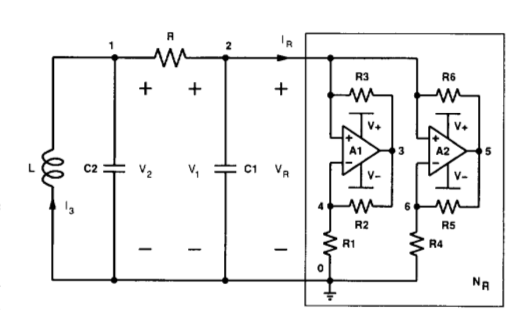
\includegraphics[scale=0.5]{imagenes/2-benford/chuas_circuit.png}
\caption{Schematic of Chua's Circuit }
\end{figure}

The dynamics of the system can be modeled by the system of three nonlinear ordinary differential equations:\\
\begin{align}
 \frac{dV_1}{dt}&=\frac{G}{C_1}(V_2-V_1)-\frac{1}{C_1}f(V_1)\\
 \frac{dV_2}{dt}&=\frac{1}{C_2}I_3-\frac{G}{C_2}(V_2-V_1)\\
 \frac{dI_3}{dt}&=-\frac{1}{L}V_2\\
\end{align}

with $G=\frac{1}{R}$ and $f(V_1)$ is given by:\\
\begin{align*}
\frac{G}{C1}V_2-\frac{G'_b}{C_1}V_1-(\frac{G_b-G_a}{C_1})E &\quad if \quad V_1< -E\\
\frac{G}{C1}V_2-\frac{G'_a}{C_1}V_1 &\quad if \quad -E\geq v1 \leq E\\
\frac{G}{C1}V_2-\frac{G'_b}{C_1}V_1-(\frac{G_a-G_b}{C_1})E &\quad if \quad V_1>E
\end{align*}
\item \textbf{Properties}
      \begin{enumerate}
       \item \textbf{Nonlinearity:} The system of equations has a nonlinear 2-terminal resistor described by a three segment piecewise-linear v-i characteristic shown in the following figure:


            \begin{figure}[h]
            \centering
            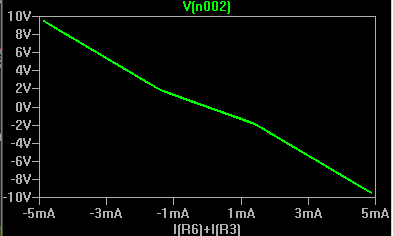
\includegraphics[scale=0.5]{imagenes/2-benford/v-i.png}
            \caption{v-i characteristic of the non-linear resistor }
            \end{figure}

      The piecewise-linear nature of the nonlinearity in Chua's Oscillator divides the state-space of the circuit into three distinct affine regions ($V_1<E$), ($\|V_1\|<E$) and ($V_1>E$)
      \item \textbf{Symmetry:}The piecewise-linear function is symmetric with respect to the origin, there exists three equilibrium points, at 0, $P_-$ and $P_+$. In the following figure, a double scroll Chua's attractor is shown. Since three equilibrium points are involved, this attractor is symmetric with respect to the origin\\

            \begin{figure}[h]
            \centering
            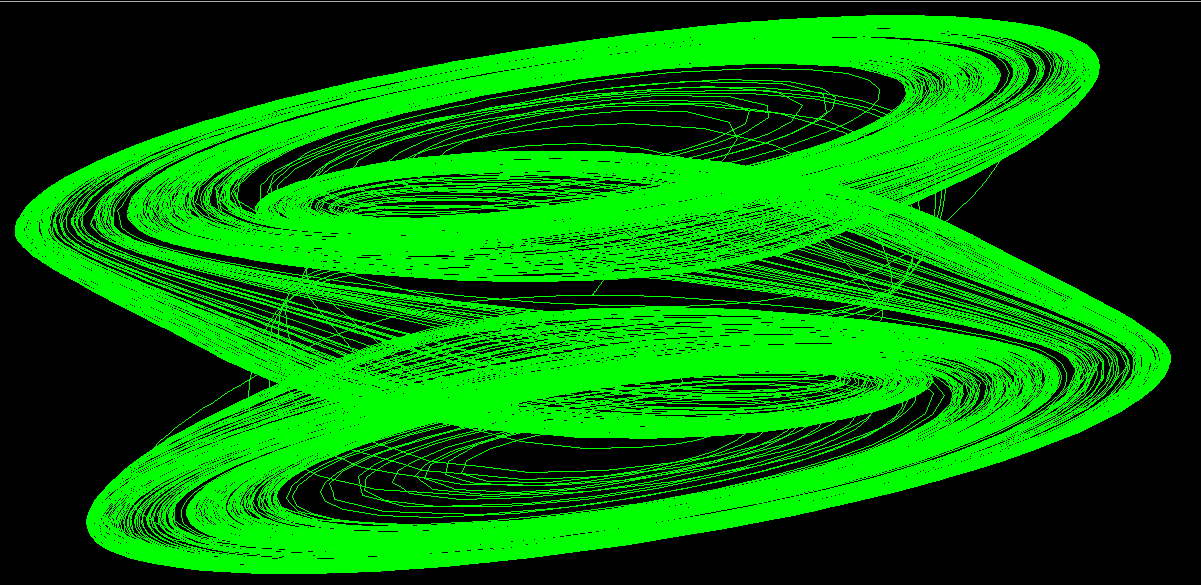
\includegraphics[scale=0.2]{imagenes/2-benford/chua_circuit.png}
            \caption{v-i characteristic of the non-linear resistor }
            \end{figure}
      \item \textbf{Dissipativity}
      \end{enumerate}
\end{itemize}
